% Generated by scripts/2026-10-21/extract_floats.py from paper/main_ko.tex; edit the full manuscript, not this file.
\begin{figure}[htbp]
\centering
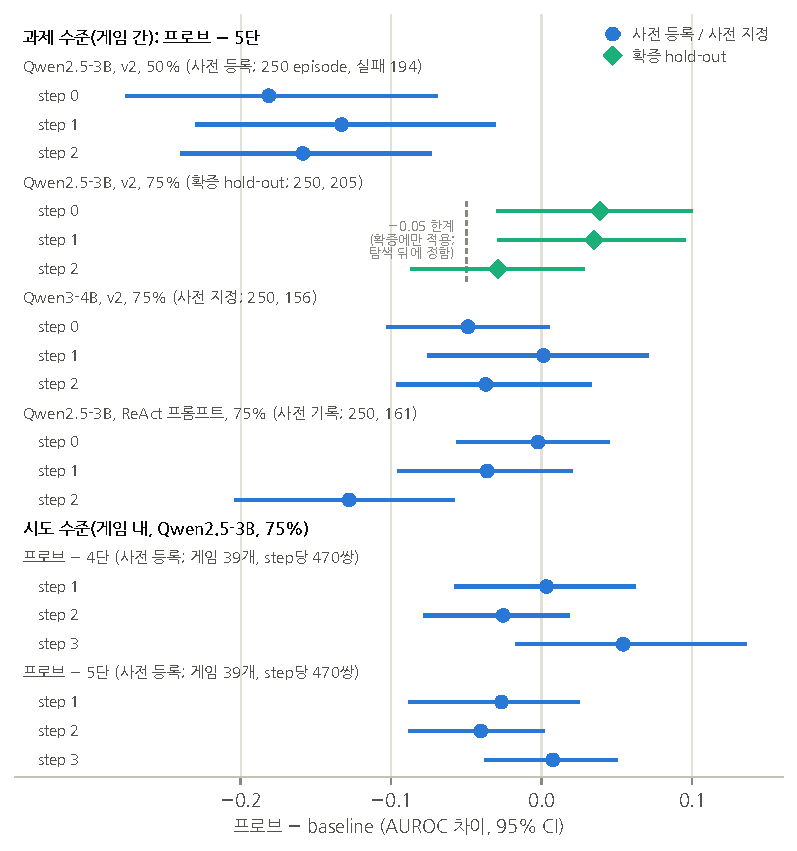
\includegraphics[width=0.82\linewidth]{fig3_probe_minus_baseline_ko.pdf}
\caption{사전 등록·사전 지정·확증 프로브 대 baseline 비교 전부(18개, 우수 0개). 이 비교들은 게임과 baseline을 공유해 독립이 아니므로, 개수는 합친 추정치가 아니다. 점은 AUROC 차이, 막대는 95\% CI. 과제 수준: 프로브 $-$ 5단, scene 단위 군집 bootstrap(1,000회), 라벨에 설정과 $n$(episode, 실패). 시도 수준: 게임 내 쌍 AUROC 차이, 게임 단위 bootstrap(1,000회). 라벨을 섞은 데이터에서 이 구간은 귀무값을 80--94\%만 포함해(\ref{sec:attempt}절) 실제보다 좁다. 점선: 비열등 한계 $-0.05$, 확증 hold-out에만 적용하며 탐색 분석 뒤에 정했다. 탐색 추정치는 넣지 않았다(그림~\ref{fig:heat}).}\label{fig:forest}
% 출처: results/probe_main_3b_primary_diff.csv, confirm_main_3b_diff.csv, task_qwen3_4b_diff_p.csv, task_react_qwen25_3b_diff_p.csv, within_game_diff.csv
\end{figure}
